
\section{Basic Models}
I want to set some baseline movement models in this section, for it not only helps me to visualize the problem, but can also test my conjuncture of the continuous approximations.

Firstly, I wish to find an optimal starting condition, and an analogy can made with projectile motion, leading to the precalculation of the vertical motion; Secondly, I hope to model the mechanics between the remaining two axis of motion; Lastly, I will fit various acceleration models using my intuition, calculus, and even polar coordinates.

% straight line
\subsection{Key idea and boundary condition}
The key idea that will be repeated throughout this analysis is the extend that maximizing the player velocity will maximize the displacement. I hypothesized this from the position differential equations in Eq. \ref{eq:1de2}, that under the assumption of constant velocity, the final displacement will be proportional to that constant:
\begin{align*}
    \tp'(t) &= \tv(t)\\
    \tp(t) &= \int \tv(t) \, dt\\
    &= t(\tv(t)) + \tp(0) = t(\tv(t)) + \tvec{0},\\
    \tp &\propto \tv(t).
\end{align*}

Therefore, I was able to set an optimal initial velocity for the player, also known as the boundary condition of the problem. For we are maximizing the jump displacement, and higher velocity equates to higher displacement, it is reasonable to set the initial velocity as high as possible. So
\[
    \tmag{\tv} = 250,
\]
where $250$ is fastest ground running speed.


\begin{figure}[H]
    \centering
    \begin{minipage}{.5\textwidth}
        \centering
        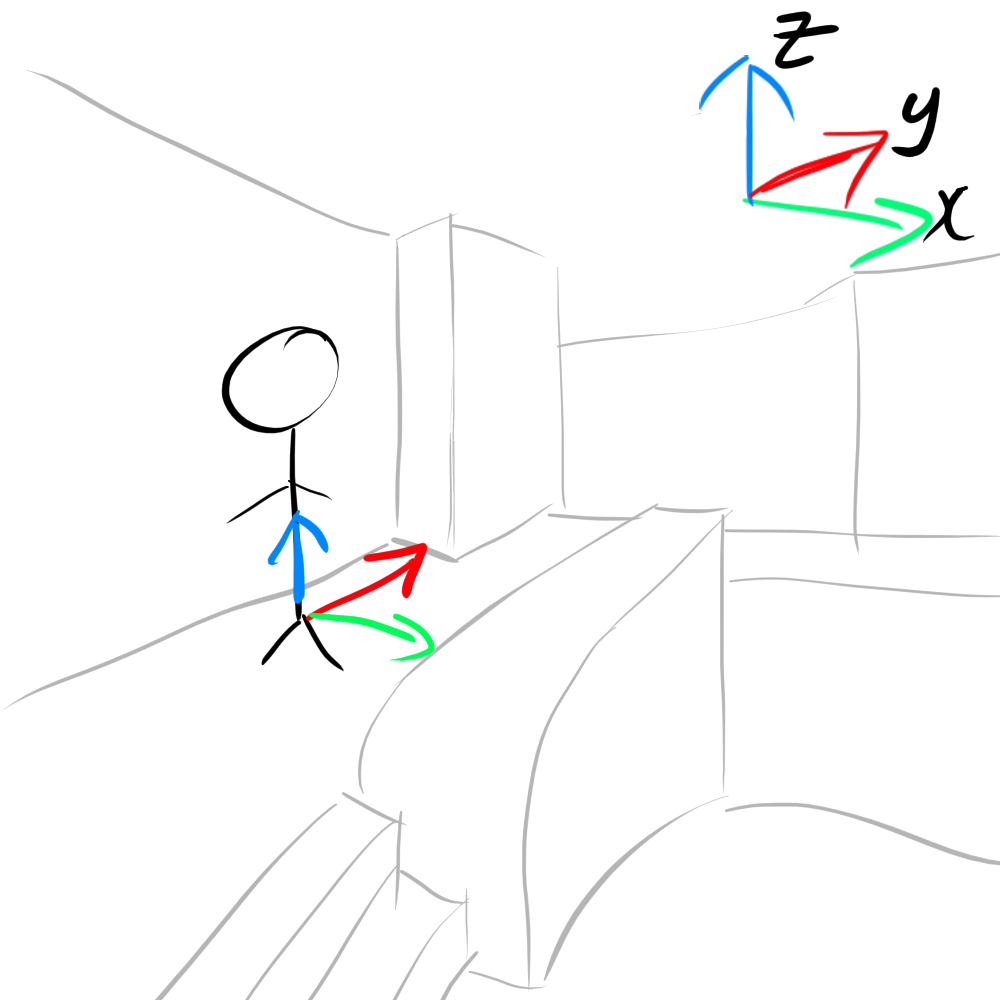
\includegraphics[width=0.9\linewidth]{assets/1coordinates.png}
        \caption{The coordinate system}
        \label{fig:1coordinates}
    \end{minipage}%
    \begin{minipage}{.5\textwidth}
        \centering
        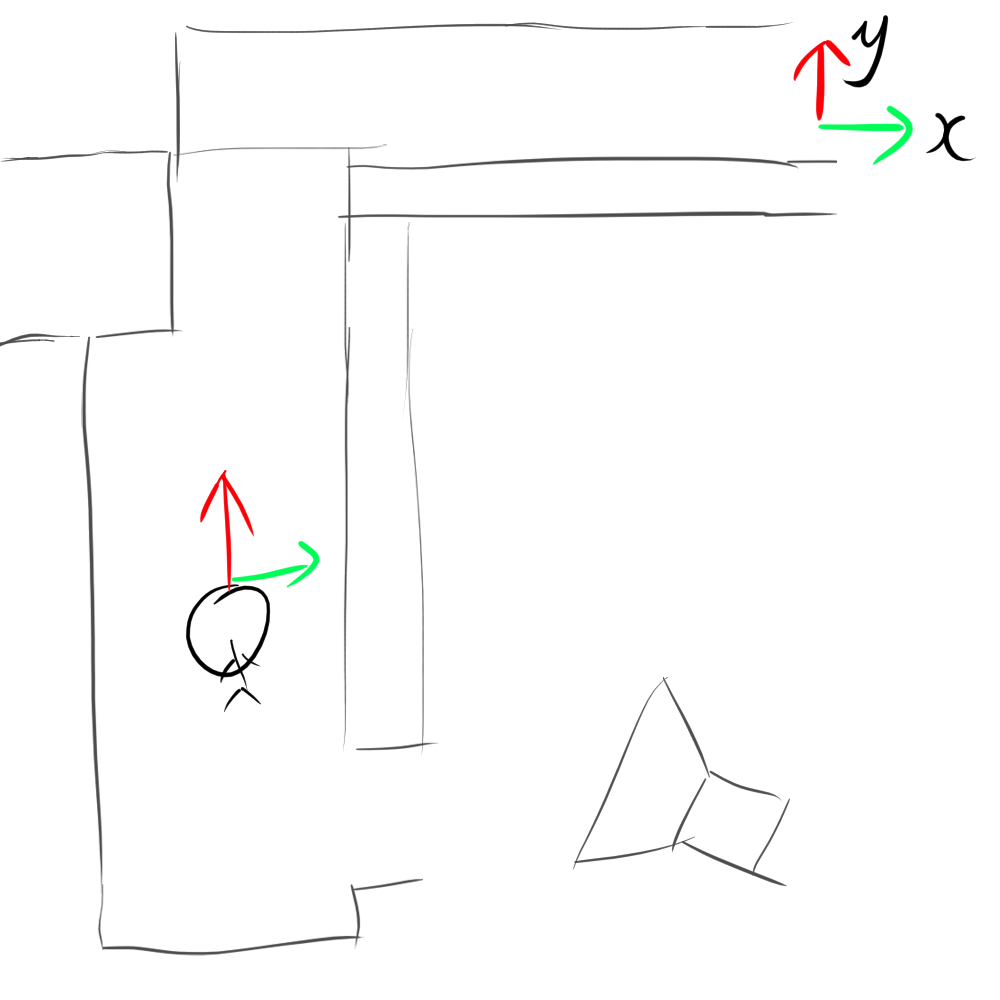
\includegraphics[width=0.9\linewidth]{assets/2coordinate_topdown.png}
        \caption{The top down view}
        \label{fig:2coordinates_topdown}
    \end{minipage}
\end{figure}


Furthermore, it should be noted that the problem is rotationally invariant when viewed top down. Let the z-axis denote the vertical height of the player, and the x,y-axis to be the plane displacement from a top down view (see figure \ref{fig:1coordinates}, figure \ref{fig:2coordinates_topdown}). \begin{wrapfigure}{r}{0.40\textwidth}
    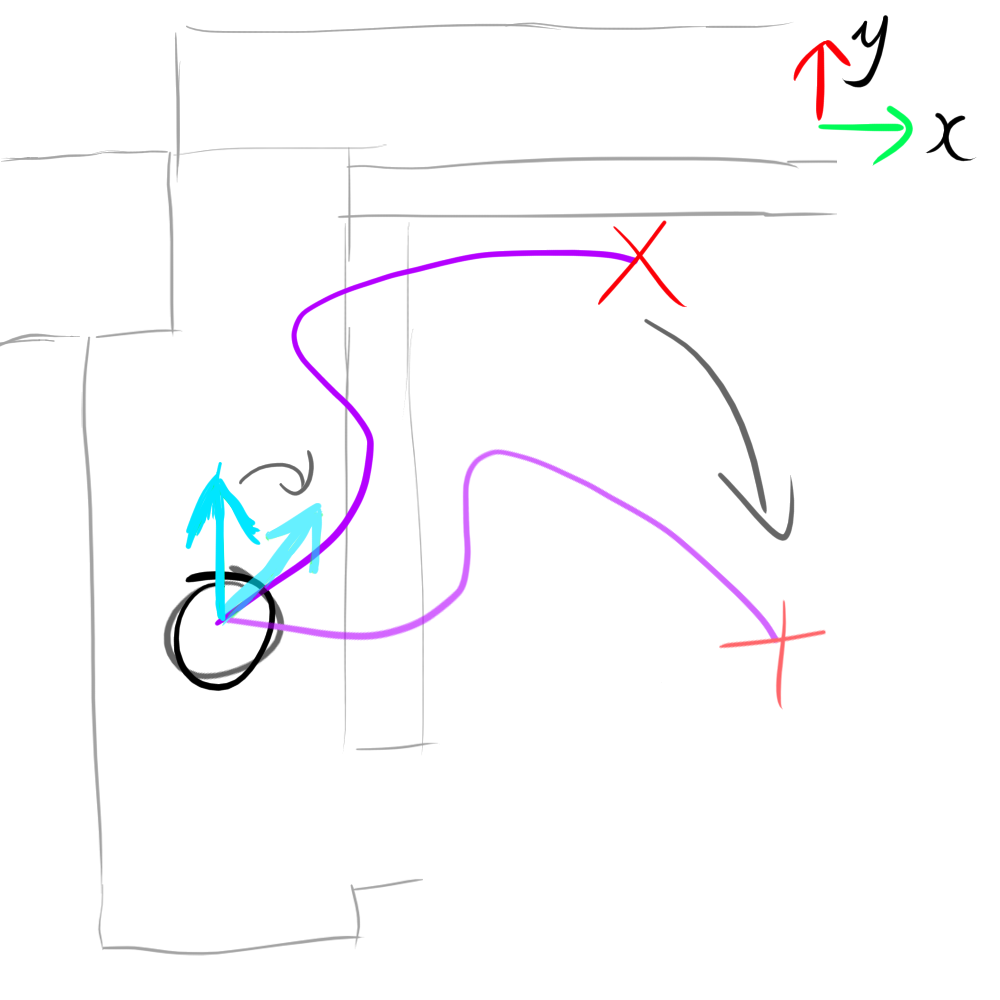
\includegraphics[width=0.37\textwidth,right]{assets/2turning.png}
    \caption{Rotational Invariant (the player wishes to go rightwards)}
    \label{fig:2turning}
\end{wrapfigure}
By considering only the x,y-axis --- and the z-axis remaining constant before and after the jump --- I realized that an optimal strategy does not depend on the angle of the initial velocity vector within the plane, for unless we somehow ended up behind our initial direction, it is always possible to rotate the initial velocity such that we travel in a desired direction of displacement (see figure \ref{fig:2turning}). This meant that the optimal initial velocity is not restricted to a certain direction, but for the sake of consistency between models, I shall use the initial velocity pointing in the y-axis:
\[
    \tv = \tang{0, 250, 0}.
\]

\subsection{Straight Line}

With the key idea and boundary condition in mind, I attempted a straight line strategy. This model has the player accelerate and move in a straight line, for mathematics has taught me that the shortest distance between two points comes from a line, resulting in less time needed to travel a long distance, which is helpful in optimizing displacement over time. To achieve this, the player would need to accelerate along the y-axis, for that is in the direction of its initial velocity, which maximizes speed at all times, and would theoretically result in the largest displacement. Mathematically, this is equivalent, to setting the directional vector to
\[
    \td(t) = \tang{0, 1, 0}
\]
for all time $t$. Realistically, this will be equivalent to pressing down ``w'' and not moving the mouse.
% do model!!
\begin{figure}[H]
    \centering
    \begin{minipage}{.5\textwidth}
        \centering
        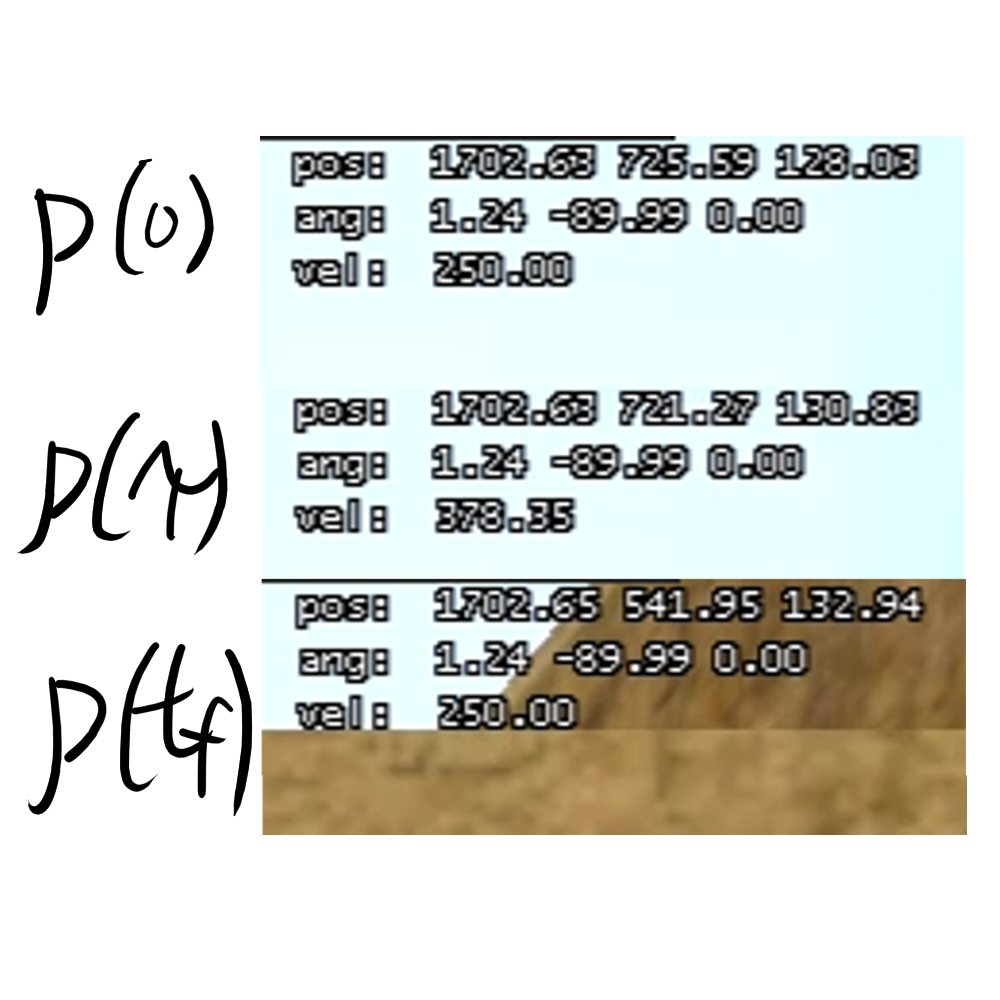
\includegraphics[width=0.9\linewidth]{assets/2straightjumping.png}
        \caption{Straight Jumping}
        \label{fig:2straightjumping}
    \end{minipage}%
    \begin{minipage}{.5\textwidth}
        \centering
        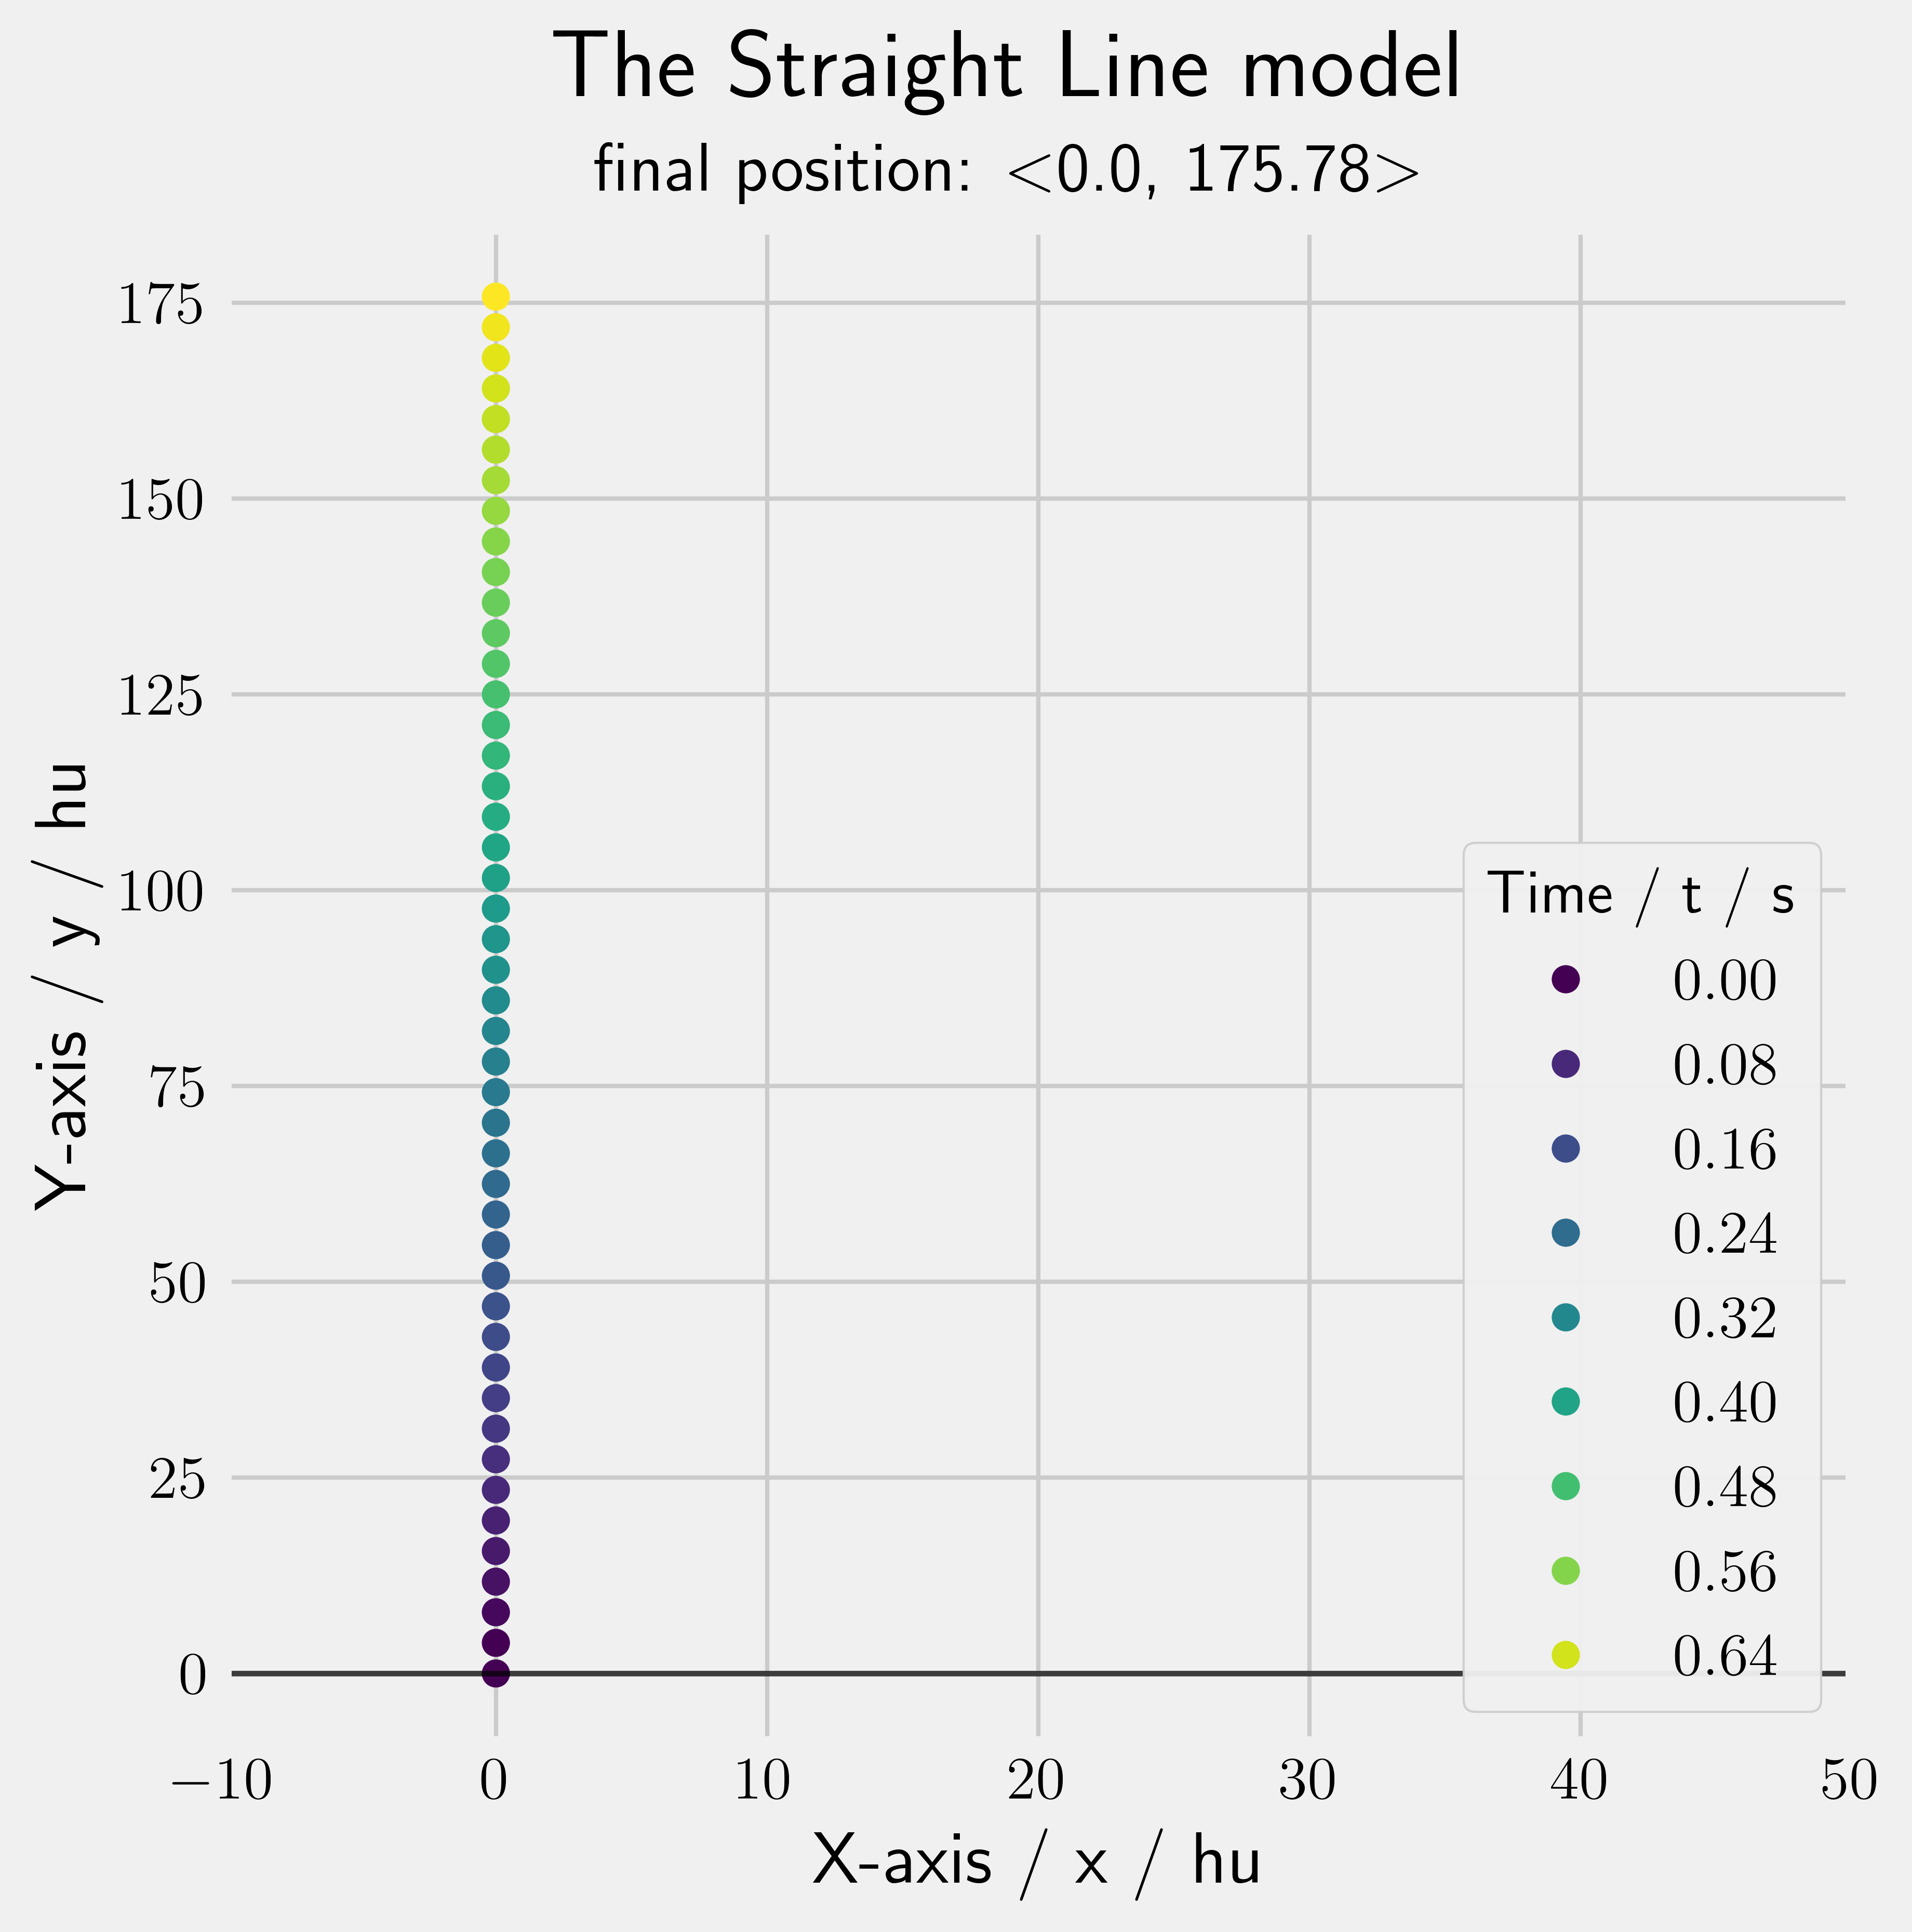
\includegraphics[width=0.9\linewidth]{assets/straight_constraint.png}
        \caption{Simulated Player Movement}
        \label{fig:straight_constraint}
    \end{minipage}
\end{figure}

To test this model, I recorded myself jumping and doing the actions described above --- it is important that the x,z-axis should not be changed after the jump; it is only the y-axis that I am recording. Figure \ref{fig:straight_constraint} shows my estimation of the real player's path with software; Figure \ref{fig:2straightjumping} shows the coordinates of the player at the start of the jump $\tp(0)$, the first discrete time of the jump $\tp(\tau)$, and the end of the jump $\tp(t_f)$ --- the symbol $t_f$ denotes the duration of the jump. Here are them written inline:
\begin{align}
 \tp(0) &= \tang{1702.63, 725.59, 128.03}, \quad \tmag{\tv(0)} = 250.00 \label{eq:2emp0}\\
 \tp(\tau) &= \tang{1702.63, 721.27, 130.83}, \quad \tmag{\tv(\tau)} = 378.35 \label{eq:2emp1}\\
 \tp(t_f) &= \tang{1702.65,541.95, 132.94}, \quad \tmag{\tv(t_f)} = 250.00 \label{eq:2emp2}.
\end{align}

\subsubsection{Analysis}
Using the simple empirical data in Eq. \ref{eq:2emp0}, Eq. \ref{eq:2emp1}, and Eq. \ref{eq:2emp2}, not only can I analyze the straight line model, but I can also calculate the various fundamental constants within the problem --- such as impulse and acceleration. However, I've also noticed that the x,z-axis has changed after the jump. The x change is likely the result of my uncertainty in having an initial velocity directly in the y-axis, but due to the rotational invariant discussed before, this is a non detrimental problem; but the z-axis is different and is likely to be the result of some ``bounciness'' of the player as it hits the floor --- which doesn't matter in the optimizing of displacement. Thus, I chose to ignore only the z-axis change during calculations.

The total displacement of this jump par definition is the expression $d = \tmag{\tp(t_f) - \tp(0)}$, which is
\begin{align*}
    d &= \sqrt{(\tp_x(t_f) - \tp_x(0))^2 + (\tp_y(t_f) - \tp_y(0))^2 + (\tp_z(t_f) - \tp_z(0))^2}\\
    &= \sqrt{(1702.65-1702.63)^2 + (541.95-725.59)^2 + (0)^2}\\
    &\approx 183.64.
\end{align*}


Firstly notice the sudden change in the velocity of the player at in first frame, time $\tau$. From this I deduced that the act of jumping is achieved by an impulse --- a sudden change in velocity --- upon the z-axis. With the assumption that no such impulses occurs in the x,y-axis, we can find the vertical change in velocity of the player at the start of the jump using the Pythagorean Theorem (figure \ref{fig:2verticalimpulse}):
\begin{wrapfigure}{r}{0.40\textwidth}
    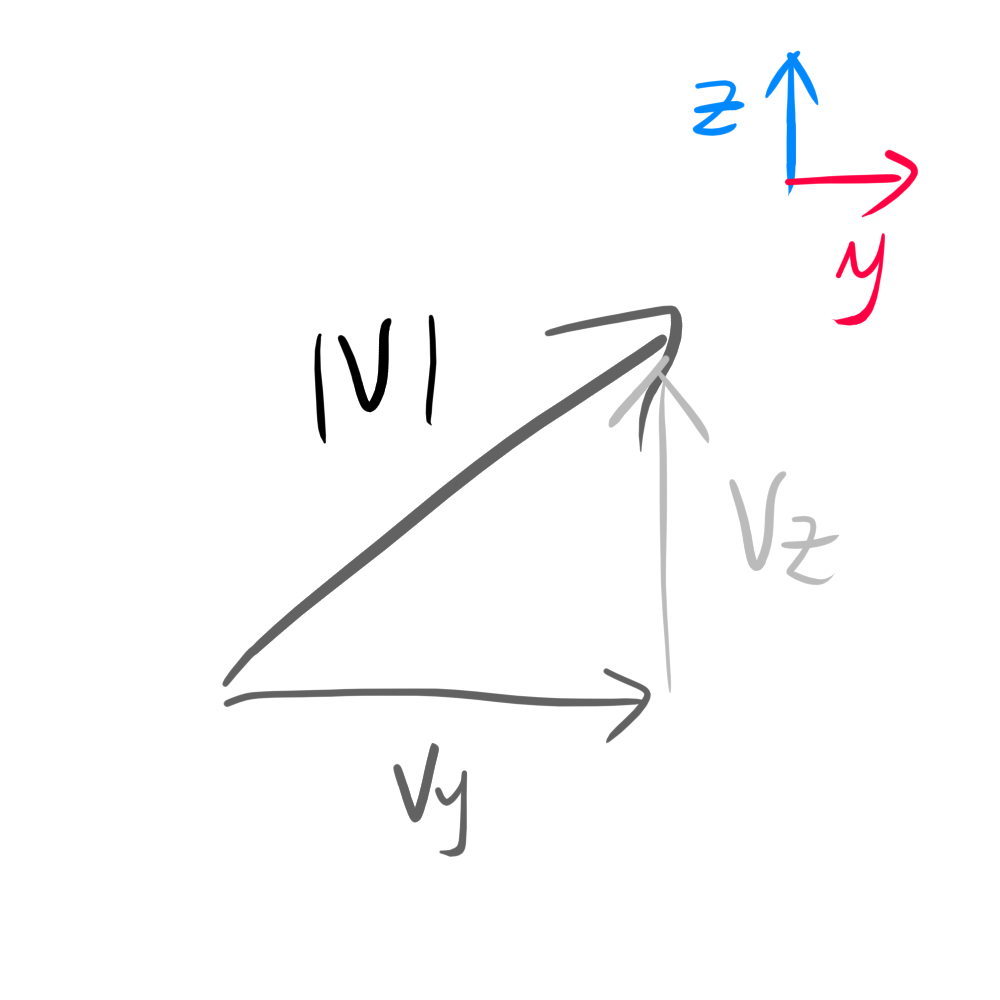
\includegraphics[width=0.37\textwidth,right]{assets/2verticalimpulse.png}
    \caption{Jumping impulses}
    \label{fig:2verticalimpulse}
\end{wrapfigure}
\begin{align*}
    \tmag{\tv}^2 &= \tv_y^2 + \tv_z^2\\
    \tv_z &= \sqrt{\tmag{\tv}^2 - \tv_y^2}\\
    &= \sqrt{378.35^2 -250^2}\\
    &= 284.00.
\end{align*}

With approximations in continuous time, we can set the player's initial vertical velocity to this number such that
\[
    \tv_{z}(0) = 284.
\]


Secondly, by measuring the duration of the jump --- which I've done by counting the number of video frames of a sixty hertz video, or $44 \times \frac{1}{60} = 0.7333 \si{s}$ --- I was able to derive the average speed $\tv_{a}$ of the player:
\[
    \tv_{a} = \frac{183.71}{0.7333} \approx 250.42.
\]

Isn't that surprising? Turns out that there is almost zero net acceleration in the straight line model --- the average velocity does not differ from its initial value --- which meant that the acceleration as a function of time $t$ and wishing direction $\td(t)$ is zero:
\[
    \ta(t, \td) = \tang{0, 0, 0}.
\]

I suspect a speed limit is in play here. This is bad in the optimization of jump displacement as it restricts the player's velocity, which by the key idea, is likely to limit the displacement too. But the game certainty cannot be limiting the magnitude of velocity directly as I've achieved higher velocity while playing, often subconsciously. My research in the engine source code \parencite{valvesoftware} and a simplified article about the mechanics in a similar game called ``Half Life'' \parencite{jwchong} was targeting exactly this mechanic of velocity limiting. In short, the player's velocity $\tv$ is limited by its projection onto the wished direction $\td$.

\subsubsection{Speed limit}
\begin{wrapfigure}{r}{0.40\textwidth}
    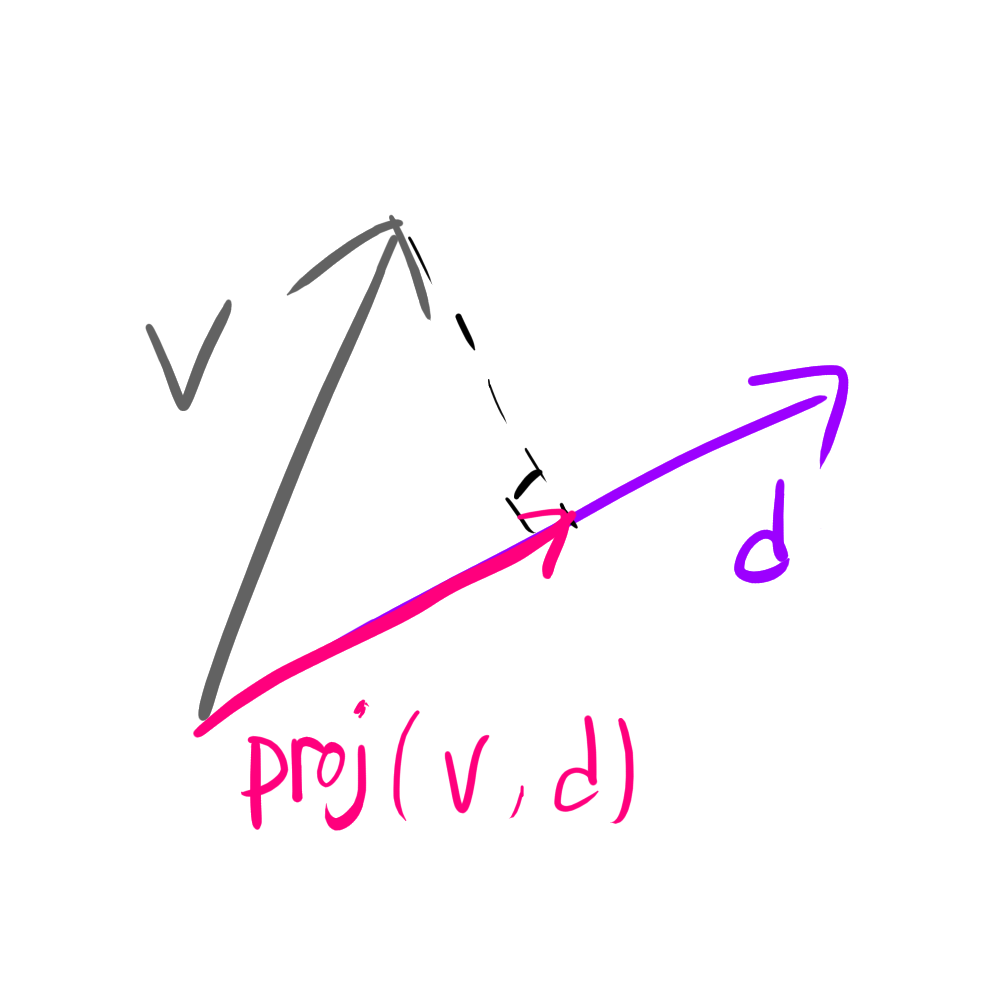
\includegraphics[width=0.37\textwidth,right]{assets/2proj.png}
    \caption{Projection limiting}
    \label{fig:2proj}
\end{wrapfigure}
A vector's projection onto another is another way to say how much the vector is pointing in the direction of another, in the form of a number. Denoted by $\text{proj}(\tv, \td)$, the projection is the side of the triangle along the direction of $\td$ form by a perpendicular line from $\tv$ to $\td$ (figure \ref{fig:2proj}). This can be defined using dot products by the following identity (APPENDIX proof):
\[
    \text{proj}(\tv, \td) = \frac{\tv \cdot \td}{\tmag{\td}}.
\]

Additionally, the game engine states that the vector $\td$ never has a z-component and is a unit vector, meaning that its magnitude is zero. Therefore the projection is simply the 2D vector dot product between $\tv$ and $\td$.
\begin{align*}
    \text{proj}(\tv, \td) &= \tv \cdot \td\\
    &= \tv_x \td_x + \tv_y \td_y + \tv_z \td_z\\
    &= \tv_x \td_x + \tv_y \td_y.
\end{align*}

Lastly, the game engine computes the player's 2D (x,y-axis) acceleration by checking if this projection excesses a limit $L$, set to $250$. If it does, acceleration will be zero; else, acceleration is a constant in the direction of $\td$, equal to $LA\tau$ in the discrete sense, and $LA$ in the continuous approximation --- where $A$ is a multiplier equal to $10$. The player's 2D acceleration function can therefore be defined piecewisely as:
\begin{figure}[H]
    \centering
    \[
        \ta(t) = \begin{cases}
            LA \td & \text{proj}(\tv, \td) < L\\
            0 & \text{otherwise}
        \end{cases}
    \]
        \caption{Player 2D acceleration function}
    \label{eq:playeracceleration}

\end{figure}

In the case of maximizing displacement, we ideally want the first condition of equation \ref{eq:playeracceleration} to be true for as long as possible. Yet in the context of my straight line model, it is simple to see that the first condition is never true, for
\begin{align*}
    \text{proj}(\tv, \td) &= \tv_x \td_x + \tv_y \td_y\\
    &= \tv_x \times 0 + \tv_y \times 1\\
    &= \tv_y,\\
    \text{and because} \quad \tv_{y}(0) &= 250 = L\\
    \text{proj}(\tv, \td) &= L\\
    \text{and} \quad \ta(t) &= 0.
\end{align*}
Our acceleration model has therefore confirmed our hypothesis that the player is not accelerating in the x,y-axis at all. This makes the model a terrible one for maximizing one's jumping displacement, as low acceleration equals to lower velocity, and in turn decreases displacement per my key idea.

\subsubsection{Continuous modeling approximation}
But before I try some other models, let's first evaluate an continuous approximation using this simplistic model.
The game engine's code reveals a gravitational acceleration $g$ --- with a value of $800$ --- on the player at all times, and I used this as an opportunity to test my continuous approximation by comparing the calculated value with the real value. Furthermore, because the z-axis acceleration is not dependent on the $\td$ --- the player's actions, we shall only attempt to model the x,y-axis actions of the player.

The objective is to solve the differential equations of motion for the player. For the x,y-axis acceleration of the player is zero, and let $g$ be the signed z-axis acceleration:
\[
    \ta = \tang{0, 0, g},
\]
the velocity as defined in Eq. \ref{eq:1de1} is the integral of acceleration --- note that $\tv_{z}(0) = 284$ as calculated before:
\begin{align*}
    \tv &= \int \ta \, dt\\
    &= \tang{0, 0, gt} + \tv(0)\\
    &= \tang{0, 250, gt + 284}.
\end{align*}

Continuing, the player position is the integral of velocity as shown in Eq. \ref{eq:1de2}. By assuming that $\tp(0) = 0$,
\begin{align*}
    \tp &= \int \tv \, dt\\
    &= \tang{0, 250t, \frac{1}{2}gt^2 + 284t} + \tp(0)\\
    &= \tang{0, 250t, \frac{1}{2}gt^2 + 284t}
\end{align*}
shows that the the y-axis displacement is $250t$. Because I've calculated the jump displacement, this means that the jump duration $t_f$ is
\[
    t_f = \frac{183.64}{250} \approx 0.735 \si{s}.
\]
Thus, since the z-axis displacement is zero, the gravitational acceleration $g$ is calculated to be
\begin{align*}
    \tp_{z}(t_f) &= \frac{1}{2}gt_f^2 + 284t_f = 0\\
    g &= - 2 \times \frac{284t_f}{t_f^2}\\
    &= -\frac{568}{t_f}\\
    &\approx -772.79.
\end{align*}

Comparing to the actual value of $g=800$, the absolute value of $772.79$ is not far off. The relative error of $\frac{800 - 772.79}{800} = 3.4\%$ is close enough for an approximation. Therefore it is justified that for the rest of the models that I can continuously use the continuous approximations, to which I will.

\subsection{Skilled Player's model}
A better strategy would be one where the player accelerates not directly along their velocity, but rather at an angle to their velocity. Personally I've been told by numerous skilled players that you need to move your mouse slowly to the right --- meaning rotating the vector $\td$ over time --- to get higher speed and distance. Now I can test this theory.

Currently, any strategy is uniquely defined by the player wishing direction function $\td(t)$. Therefore let
\[
    \td(t) = \tang{x(t), y(t)}
\]
where $x(t)$ and $y(t)$ are the x,y-components of the function. Ideally, this vector should be y-axis pointing at $t=0$, and rotate clockwise overtime as to create acceleration rotation. This reminded me of a unit circle, albeit with the x,y-axis switched, creating
\[
    \td(t) = \tang{\sin(t), \cos(t)}.
\]
One can verify that this definition both denote rotation overtime and have a magnitude of $1$. Furthermore, I can encode the rate of rotation by scaling the inner $t$ in the two trig functions by the same factor $w$, without changing its magnitude. Therefore the player direction function $\td(t)$ as recommended by skilled players is
\[
    \td(t) = \tang{\sin(wt), \cos(wt)}.
\]

My task is to find the best constant $w$ that maximizes this function. The plan is to solve the x,y-axis differential equation into a function of position $\tp$, then explicitly writing the speed limit as an inequality constraint, and finally selecting the constant $w$ that (hopefully) satisfies the constraint and maximizes the displacement.

\subsubsection{Displacement equation}
The key idea suggests that I should maximize the velocity, and as explained in the previous subsection, this meant that player acceleration $\ta$ is to be maximized by fulfilling the inequality projection in equation \ref{eq:playeracceleration}. Thus by assumption that this inequality is held,
\[
    \ta(t) = LA\td.
\]

Let $k=LA$. Notice that the velocity is the integral of acceleration; we also have to satisfy the initial velocity at $t=0$. So,
\begin{align*}
    \tv(t) &= \int \ta \, dt\\
    &= \int k \tpar{\sin(wt)}{\cos(wt)} \, dt\\
    &= \frac{k}{w} \tpar{-\cos(wt)}{\sin(wt)} + c,\\
    \tv(0) &= \frac{k}{w} \tpar{-\cos(0)}{\sin(0)} + c\\
    c &= \frac{k}{w} \tpar{1}{0} + \tpar{\tv_x(0)}{\tv_y(0)}.
\end{align*}

And the position is the integral of velocity. Again, assuming that the initial displacement is $0$. So,
\begin{align*}
    \tp(t) &= \int \tv \, dt\\
    &= \int \frac{k}{w} \tpar{-\cos(wt)}{\sin(wt)} + \frac{k}{w}\tpar{1}{0} + \tpar{\tv_x(0)}{\tv_y(0)} \, dt\\
    &= \frac{-k}{w^2} \tpar{\sin(wt)}{\cos(wt)} + \frac{k}{w}\tpar{t}{0}  + t\tpar{\tv_x(0)}{\tv_y(0)} + c.
\end{align*}

To find the integration constant $c$, consider the x-axis displacement function
\begin{align*}
    \tp_x(t) &= \frac{-k}{w^2} \sin(wt) + t\tv_x(0) + t\tv_x(0) + c_x = 0\\
    c_x &= 0,
\end{align*}
and the y-axis displacement function
\begin{align*}
    \tp_y(t) &= \frac{-k}{w^2} \cos(wt) + t\tv_y(0) + c_y = 0\\
    c_y &= \frac{k}{w^2}.
\end{align*}

Using the Pythagorean Theorem, the magnitude of the player's displacement using this model after a jump --- where $t=t_f$ --- is:
\begin{figure}[H]
    \centering
    \begin{align*}
        \tmag{\tp(t_f) - \tp(0)} &= \sqrt{\tp_x(t_f)^2 + \tp_y(t_f)^2}\\
        &= \sqrt{\left(\frac{-k}{w^2}\sin(wt_f) + t_f\frac{k}{w} \right)^2 + \left( \frac{-k}{w^2}\cos(wt_f) + 250t_f + \frac{k}{w^2} \right)^2}
    \end{align*}
    \caption{Skilled Displacement}
    \label{eq:2skilled_displacement}

\end{figure}

\begin{figure}[H]
    \centering
    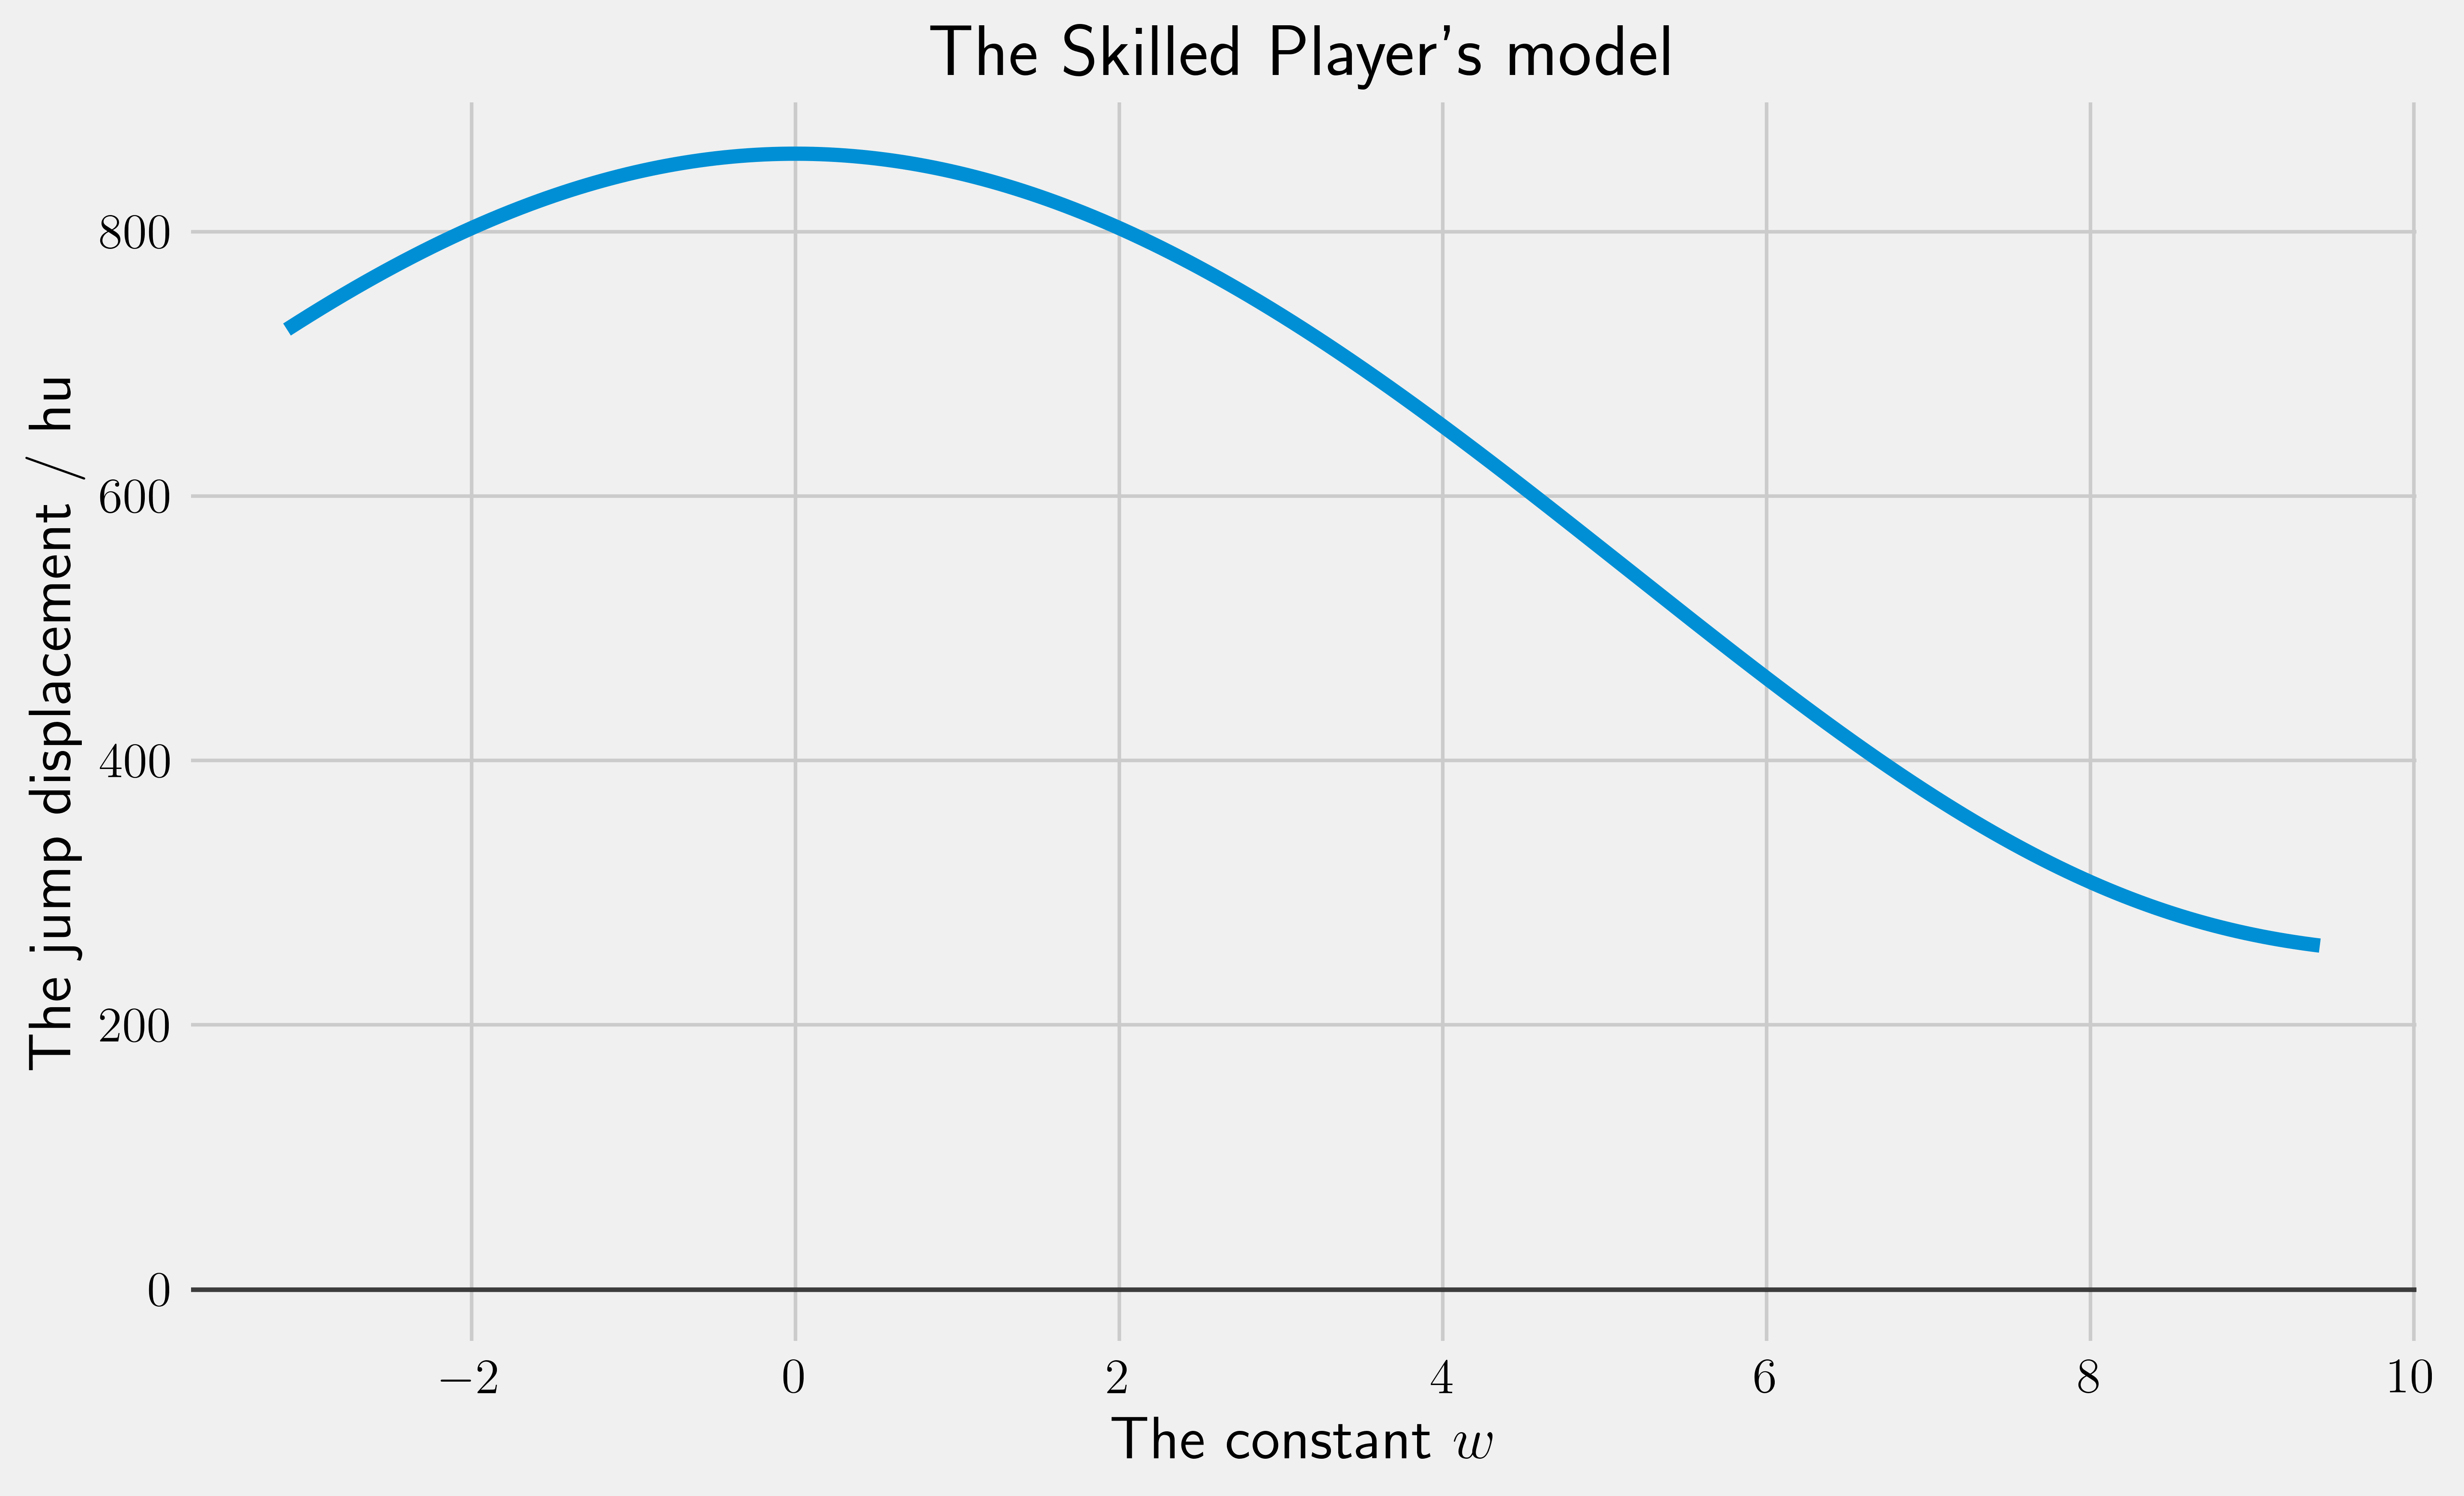
\includegraphics[width=0.85\textwidth]{assets/skilled_displacement.png}
    \caption{}
    \label{fig:skilled_displacement}

\end{figure}
The graph of equation \ref{eq:2skilled_displacement}, shown in figure \ref{fig:skilled_displacement}, is symmetrical along the y-axis. This is because of yet another symmetry between a left-turning and a right-turning jump. Quantitatively, this ``unlimited'' strategy peeks when $w=0$, where the strategy collapses to my straight line model. As the turning speed $w$ increases, the ideal displacement decreases and levels near $w=10$: I guess that a spinning player does not contribute much to jumping far. Therefore we need to choose the smallest $w$ possible to maximize potential jump displacement.

\subsubsection{Restriction equation}
In addition to finding the ``unlimited'' displacement of the strategy for all constants $w$, we also need check if they satisfy the assumption of unrestricted acceleration at all times. Ideally there should be a value of $w$ that always fits this constraint, but the smallest ``error'' from the ideal is always a backup option.

As shown in figure \ref{eq:playeracceleration}, for maximum acceleration of $\ta(t) = LA\td$, the constraint
\[
    \text{proj}(\tv, \td) < L
\]
must be held for the duration of the jump from $t=0$ to $t=t_f$. Expanding and organizing this inequality yields
\begin{align*}
    L &> \text{proj}(\tv, \td)\\
    &> \tv_x \td_x + \tv_y \td_y\\
    &> \left(-\frac{k}{w} \cos(wt) + \frac{k}{w}\right) \sin(wt) + \left(\frac{k}{w} \sin(wt) + 250\right) \cos(wt),\\
    0 &> \left(-\frac{k}{w} \cos(wt) + \frac{k}{w}\right) \sin(wt) + \left(\frac{k}{w} \sin(wt) + 250\right) \cos(wt) - 250
\end{align*}

To find the value of the constant $w$ that best fulfills this inequality, I need a quantitative measure on how well this inequality is held through the jump. Ideally the function should only include the failures of fulfilling the inequality, but as explained in the more advanced models --- that the projection RHS should be as close to zero as possible for high speeds --- I chose an integral from $t=0$ to $t=t_f$ on the absolute values of the RHS, denoted as the ``error'' of a model. This is done with the absolute function $|x|$ defined by
\[
 |x| = \begin{cases}
         x & x \geq 0\\
         -x & x < 0
        \end{cases}
\]

as to make all errors positive. Therefore the error function $R(w)$ for each constant $w$ is the integral of the absolute value of the RHS over the jump:
\begin{figure}[H]
 \centering
 \[
  R(w) = \int_0^{t_f} \left|\left(-\frac{k}{w} \cos(wt) + \frac{k}{w}\right) \sin(wt) + \left(\frac{k}{w} \sin(wt) + 250\right) \cos(wt) - 250\right| \, dt
 \]
 \caption{The error function}
 \label{eq:2error}
\end{figure}


\begin{figure}[H]
 \centering
 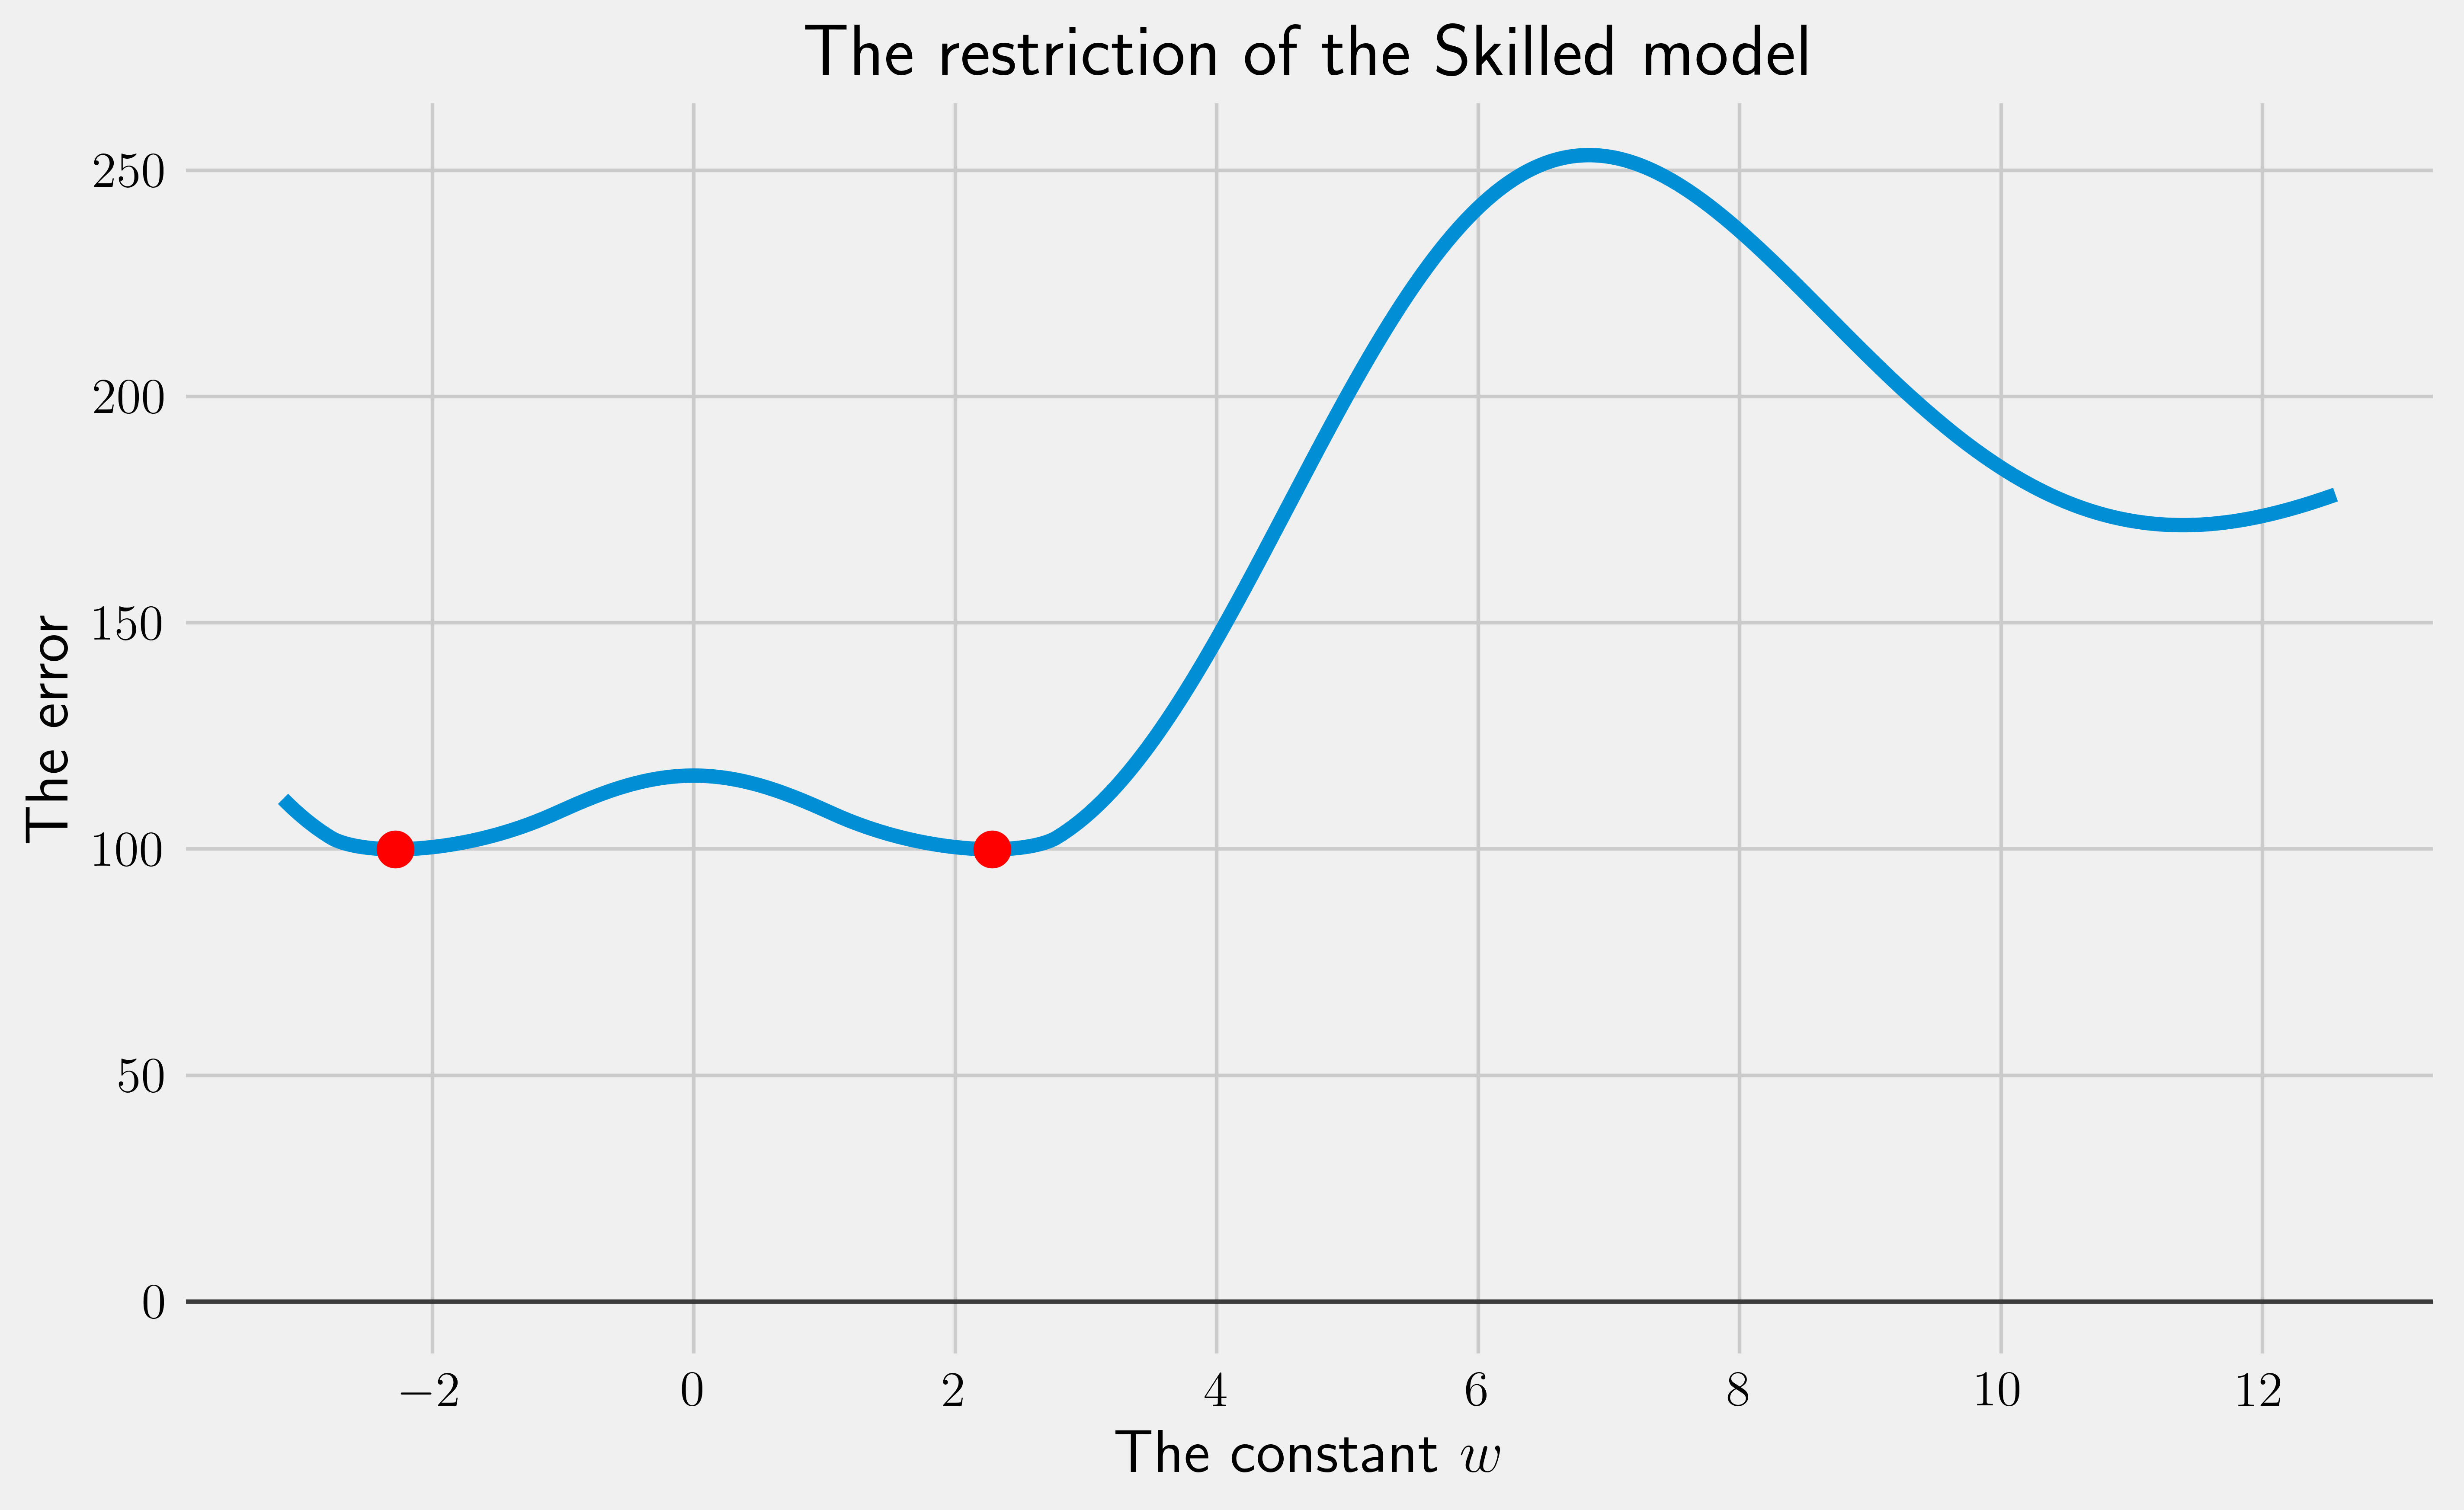
\includegraphics[width=0.85\textwidth]{assets/restriction_equation.png}
 \caption{}
 \label{fig:2error}
\end{figure}
% TODO: if needed, show the two red dots and choose the smallest one
Figure \ref{fig:2error} shows the graph of the error function in equation \ref{eq:2error}. While it may be possible to find the minimum of the error function using calculus, the steps are too complex and a numerical is taken instead and is shown by the red dot in the graph.

\begin{wrapfigure}{r}{0.50\textwidth}
    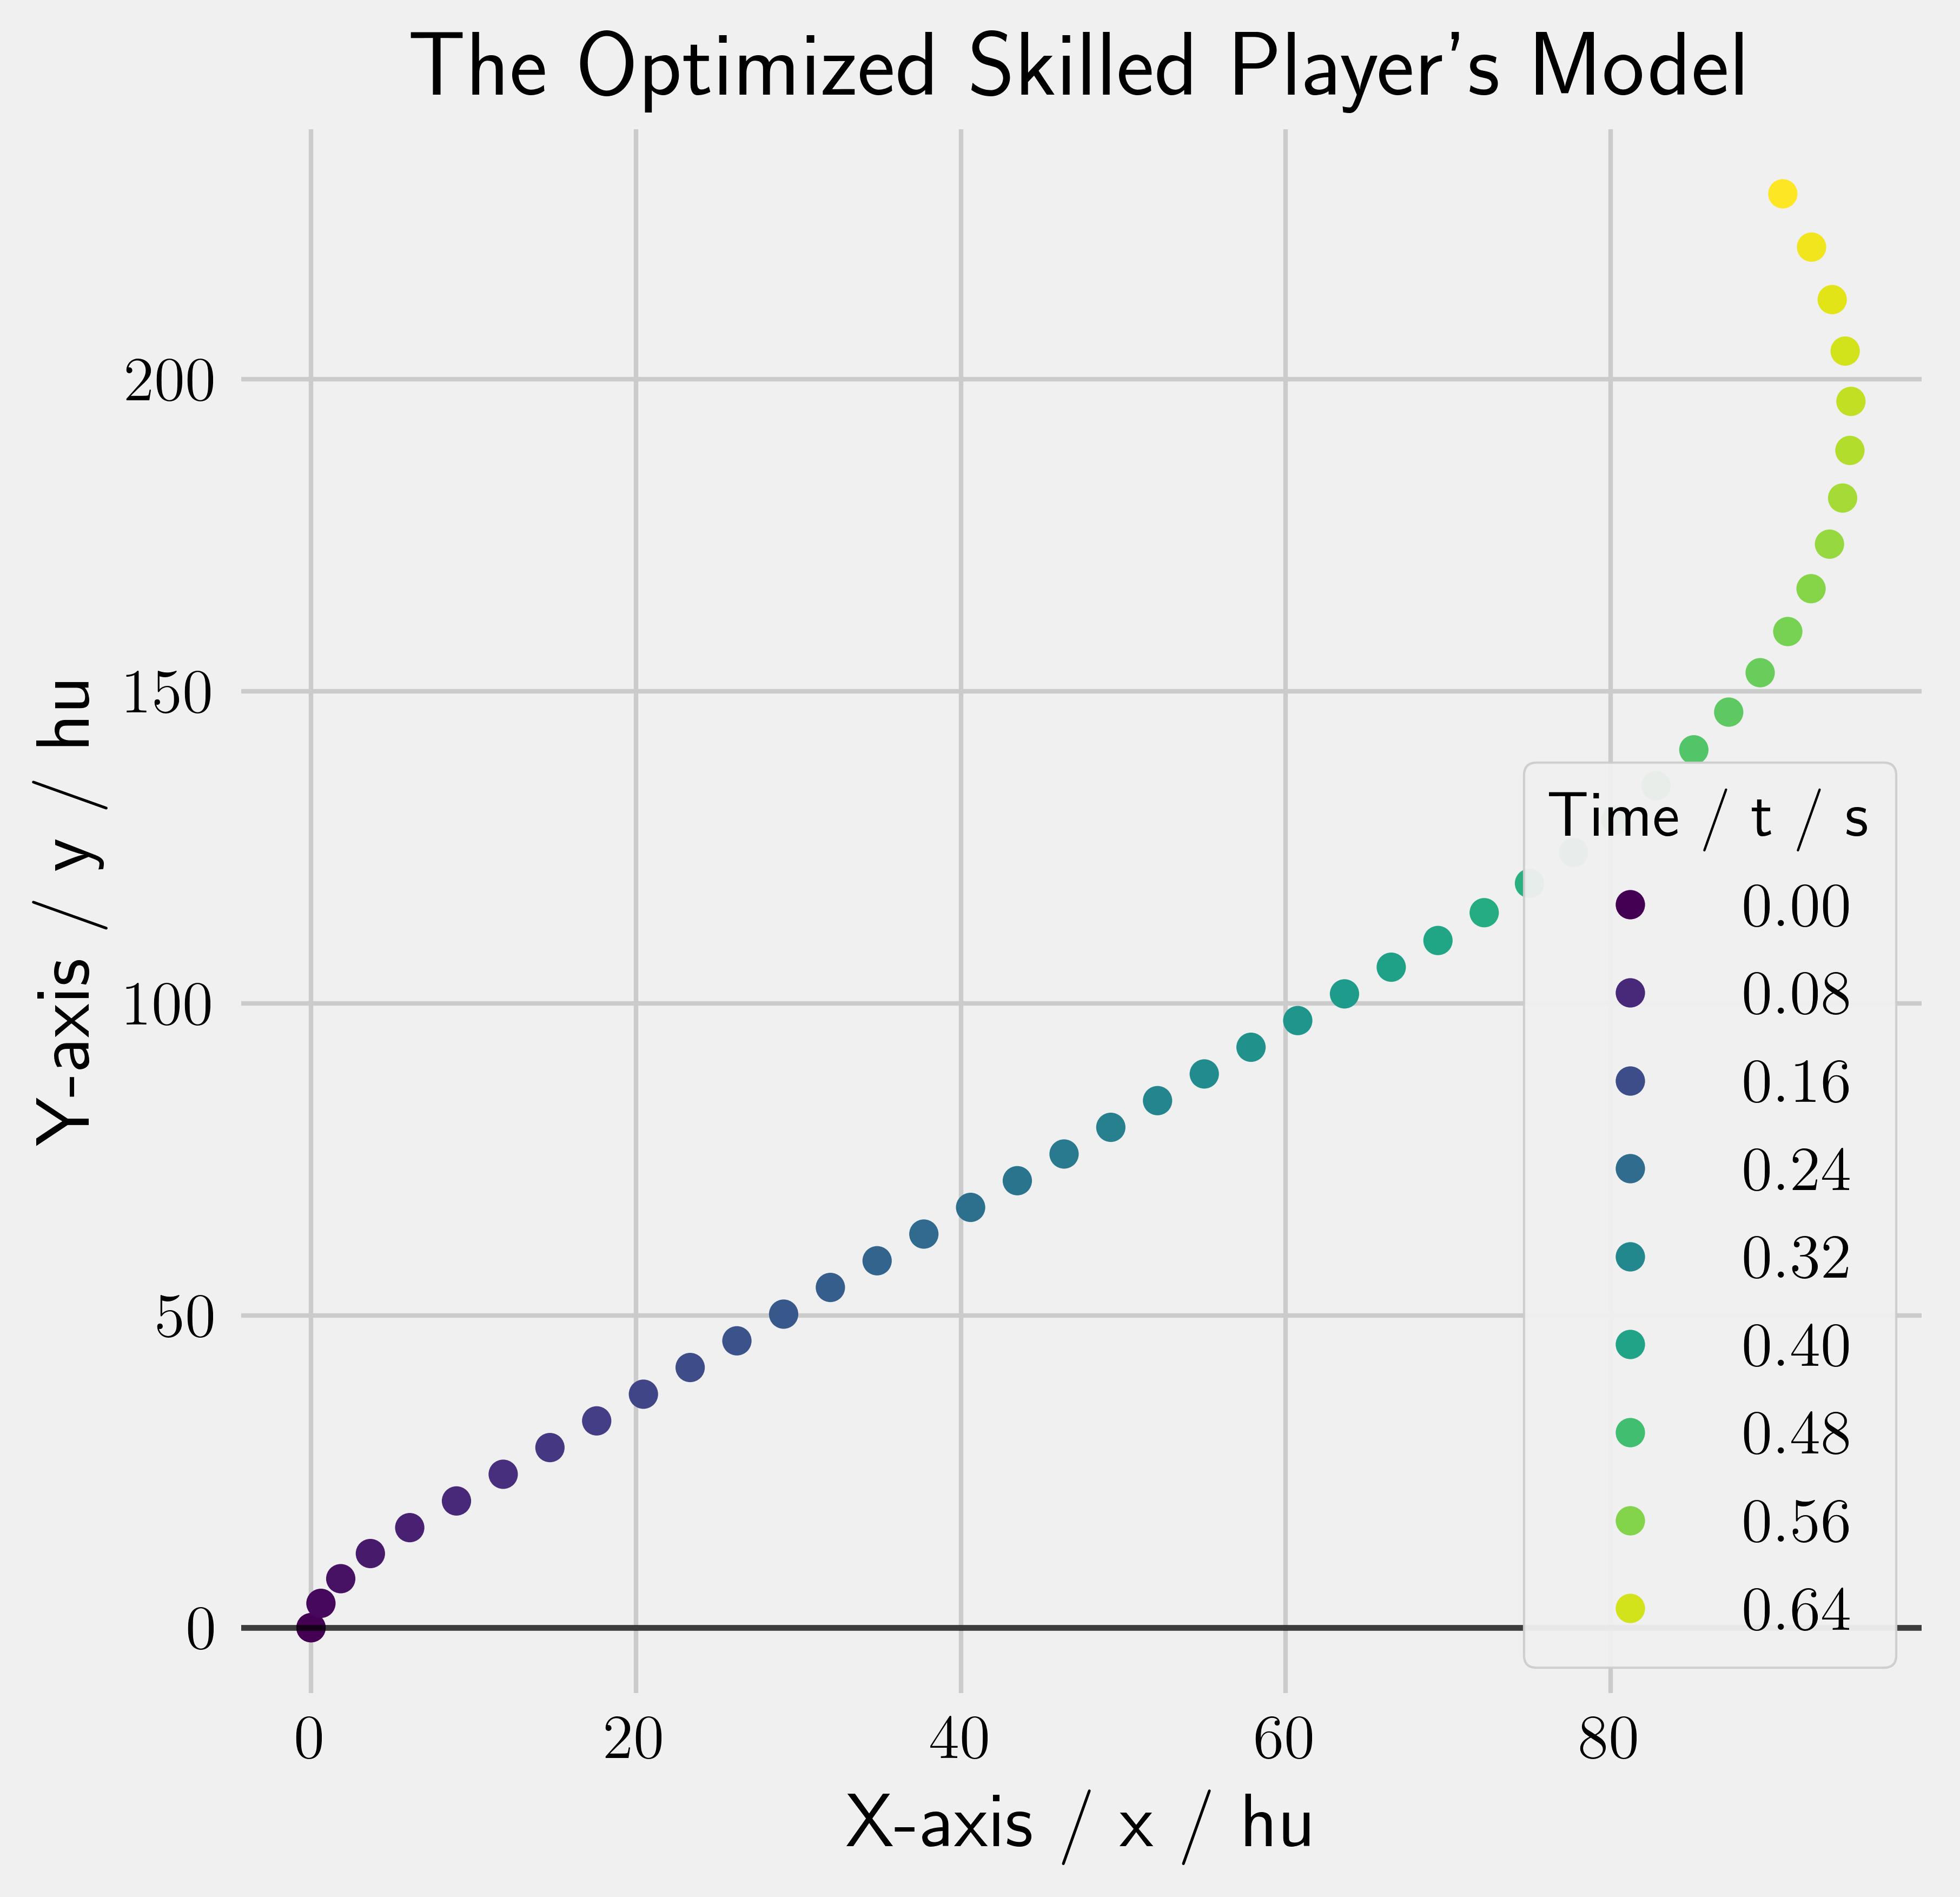
\includegraphics[width=0.47\textwidth,right]{assets/skilled_player.png}
    \caption{Skilled Player's Model}
    \label{fig:skilled_player}
\end{wrapfigure}

My program shows that the red dot is at coordinate
\[
    \tang{4.2884, 184.4228},
\]
meaning that the error function is the smallest in this skilled strategy with a constant $w=4.2884$. So the skilled player's model is defined by the direction function
\[
    \td(t) = \tang{\sin(4.2884t), \cos(4.2884t)},
\]
indicating a relatively fast rate of turning at a period of $\frac{2\pi}{4.2884} = 1.4652\si{s}$.


Ideally, this optimized model corresponds to a displacement of $627.35$ using figure \ref{fig:skilled_displacement}. But I suspect the leftover ``$184.4228$'' errors to decrease the displacement by quite an amount. Figure \ref{fig:skilled_player} shows the actual path of the player when simulated in game; this is in combination with a correctly estimated lower displacement of $254.19$ units.
\begin{align*}
    \tp(t_f) &= \tang{88.3021, 238.3556}\\
    \tmag{\tp(t_f)} &\approx 254.19
\end{align*}

The skilled player's model does indeed produce a higher displacement ($254.19$) than the straight line model ($183.64$). Not only does this confirm the theory from these skilled people, but the large error of the even optimized model could indicate further possible optimizations when I look at the problem discretely.
